Интегральное представление гармонических функций является основным аппаратом для изучения свойств гармонических функций. Одним из важнейших следствий интегральной формулы является принцип максимального значения, часто используемый при решении краевых задач и доказательстве теоремы единственности. \\

\subsubsection{Вывод формул}
Формулы Грина являются прямым следствием формулы Остроградского.
	Формула Остроградского в простейшем случае имеет вид

\begin{equation}
	\iiint\limits_W \derp{R}{z}{}\, dx\, dy\, dz = \iint\limits_S R \cos \gamma\, d\sigma
	\label{equ:equOstrograd}
\end{equation}
где $W$ -- некоторый объём, ограниченный достаточно гладкой поверхностью $S$, $R(x, y, z)$ -- произвольная функция, непрерывная внутри $W + S$ и имеющая непрерывные производные внутри $W$, $\gamma$ -- угол между направлением оси $z$
 и внешней нормалью к $S$. В справедливости этой формулы нетрудно убедиться, проинтегрировав по $z$.\\

    Формулу Остроградского обычно записывают в виде
\begin{equation}
	\iiint\limits_W\left( \derp{a_x}{x}{} + \derp{a_y}{y}{} + \derp{a_z}{z}{}\right) \, d \tau = \iint\limits_S \left\{ a_x \cos \alpha + a_y \cos \beta + a_z \cos \gamma \right\} \, d \sigma
	\label{equ:equOstrograd2}
\end{equation}

	Если $a_x, a_y, a_z$ рассматривать как компоненты некоторого вектора $A = a_x i + a_y j + a_z k$, то формулу Остроградского \eqref{equ:equOstrograd2} можно записать следующим образом
\begin{equation} 
	\iint\limits_W \mathrm{div} \, A \, d \tau = \iint\limits_S A_n \, d \sigma
	\label{equ:equOstrograd3}
\end{equation}
где
 \[
	\mathrm{div}  \bar A = \derp{a_x}{x}{} + \derp{a_y}{y}{} + \derp{a_z}{z}{}
\]
и
\[	
	A_n = a_x \cos \alpha + a_y \cos \beta + a_z \cos \gamma
\]
-- составляющая вектора $A$ вдоль внешней нормали.\\

Перейдём к выводу формул Грина.\\
Пусть $u = (x, y, z)$ и $v = v(x, y, z)$ -- функции. непрерывные вместе со своими первыми производными внутри $W + S$ и имеющие непрерывные вторые производные внутри $W$.

Полагая
\[
	a_x = u \derp{v}{x}{} \quad	a_y = u \derp{v}{y}{} \quad a_z = u \derp{v}{z}{}
\]
и пользуясь формулой Остроградского \eqref{equ:equOstrograd3}, приходим к так называемой \textit{первой формуле Грина}
\begin{equation}
	\iiint\limits_W u \Delta v \, d\tau = \iint\limits_S \derp{v}{n}{} \, d \sigma - \iiint\limits_W \left( \derp{u}{x}{} \derp{v}{x}{} + \derp{u}{y}{} \derp{v}{y}{} + \derp{u}{z}{} \derp{v}{z}{}\right)\, d \tau
\end{equation}
где $\Delta = \derp{}{x}{2} + \derp{}{y}{2} + \derp{}{z}{2}$ -- оператор Лапласа, $\derp{}{n}{} = \cos \alpha \derp{}{x}{} + \cos \beta \derp{}{y}{} + \cos \gamma \derp{}{z}{}$ -- производная по направлению внешней нормали.
	Если учеcть соотношение
\[
	\mathrm{grad}\,u\, \mathrm{grad}\, v = \nabla u \cdot \nabla v = \derp{u}{x}{} \derp{v}{x}{} + \derp{u}{y}{} \derp{v}{y}{} + \derp{u}{z}{} \derp{v}{z}{}
\]
то формулу Грина можно представить в виде
\[
	\iiint\limits_W u \Delta v \, d \tau = - \iiint\limits_W \nabla u \nabla v \, d \tau + \iint\limits_S u \derp{v}{n}{} \, d \sigma
\]
Меняя местами функции $u$ и $v$, будем иметь
\[
	\iiint\limits_W v \Delta u \, d \tau = - \iiint\limits_W \nabla v \nabla u \, d \tau + \iint\limits_S v \derp{u}{n}{} \, d \sigma
\]
Вычитая эти равенства, получаем \textit{вторую формулу Грина}
\begin{equation}
			\iint\limits_S \left(u \der{v}{n}{} - v \der{u}{n}{}\right) d\sigma = \iiint\limits_{W} \left(u \Delta v - v \Delta u \right) d \tau
	\label{equ:Green1}
\end{equation}\\
%\[
%	\bar A = u \left(\derp{v}{x}{} \vec i + \derp{v}{y}{} \vec j + \derp{v}{z}{} \vec k \right) - v \left(\derp{v}{x}{} \vec i + \derp{v}{y}{} \vec j + \derp{v}{z}{} \vec k \right) =			\left(u \derp{v}{x}{} - v \derp{u}{x}{} \right) \vec i + \left(u \derp{v}{y}{} - v \derp{u}{y}{} \right) \vec j + \left(u \derp{v}{z}{} - v \derp{u}{z}{} \right) \vec k
%\]
%\[
%	div A = \derp{}{x}{} \left(u \derp{v}{x}{} - v \derp{u}{x}{} \right) \vec i + \derp{}{y}{} \left(u \derp{v}{y}{} - v \derp{u}{y}{} \right) + \derp{}{z}{} \left(u \derp{v}{z}{} - v \derp{u}{z}{} \right) = 			u \left( \derp{v}{x}{2} + \derp{v}{y}{2} + \derp{v}{z}{2}\right) - v  \left( \derp{u}{x}{2} + \derp{u}{y}{2} + \derp{u}{z}{2}\right) + \derp{u}{y}{}\derp{v}{x}{} - \derp{v}{x}{} \derp{u}{y}{} + \derp{u}{y}{} \derp{v}{y}{} - \derp{v}{y}{} \derp{u}{y}{} + \derp{u}{z}{} \derp{v}{z}{} - \derp{u}{z}{} \derp{v}{z}{}
%\]
		%Получили формулы Грина:\\
Основная интегральная формула Грина
\begin{equation}
	\Omega \cdot u(A) = \iint\limits_S \left[ \frac{1}{R_{AP}} \derp{u(P)}{n_P}{}  - u (P) \derp{}{n_P}{} \left( \frac{1}{R_{AP}} \right) \right] d\sigma_P - \iiint\limits_W \frac{\Delta u (P)}{R_{AP}}\, d\tau_P
	\label{equ:equMainGreen3d}
\end{equation}
где $\Omega$ принимает значения 

\[
	\Omega = \begin{cases}
		4 \pi &\mbox{если точка}\, A\, \mbox{лежит внутри}\, W\\
		2 \pi &\mbox{если точка}\, A\, \mbox{лежит на границе}\, S\\
		0 & \mbox{если точка}\, A\, \mbox{лежит вне}\, W
	\end{cases}
\]


Аналогичная формула существует и для гармонических функций двух независимых переменных. 
Пусть $S$ -- область на плоскости $(x, y)$, ограниченная контуром $C$, а $n$ -- направление нормали к этому контуру, внешнее по отношению к области $S$.

Полагая во второй формуле Грина $v = \ln \frac{1}{R_{AP}}$, где $R_{AP} = \sqrt{ (x - x_0)^2 + (y - y_0)^2}$ -- расстояние $P$ от $A$, получаем 
\begin{equation}
	\Omega \cdot u(A) = \int\limits_S \left[ \ln \frac{1}{R_{AP}} \derp{u(P)}{n_P}{}  - u (P) \derp{}{n_P}{} \left( \ln \frac{1}{R_{AP}} \right) \right] dS_P - \iint\limits_S \frac{\Delta u (P)}{\ln R_{AP}}\, dS_P
	\label{equ:equMainGreen2d}
\end{equation}
где $\Omega$ принимает значения 

\[
	\Omega = \begin{cases}
		2 \pi &\mbox{если точка}\, A\, \mbox{лежит внутри}\, S\\
		\pi &\mbox{если точка}\, A\, \mbox{лежит на границе}\, C\\
		0 & \mbox{если точка}\, A\, \mbox{лежит вне}\, S
	\end{cases}
\]


\subsubsection{Метод Грина для задачи Дирихле в трёхмерном случае}\label{que:25}
	Вторая формула грина:
\[ 
			\iint\limits_S \left(u \der{v}{n}{} - v \der{u}{n}{}\right) d\sigma = \iiint\limits_{W} \left(u \Delta v - v \Delta u \right) d \tau
\]
Рассмотрим трёхмерную задачу Дирихле. 
\[
	\Delta u = 0
\]
\[
	u\big|_S = f
\]
\begin{wrapfigure}{r}{0.3\textwidth}
	\centering
	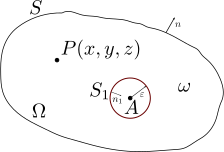
\includegraphics[width = 0.3\textwidth]{figGreenThreeDim.pdf}
\end{wrapfigure}
Применим вторую формулу Грина к этой задаче.\\

В области $\Omega$ возьмём $(\cdot)A(x_0, y_0, z_0)$ и произвольную $(\cdot)P(x, y, z)$.
\[
	r_{AP} = \sqrt{(x - x_0)^2 + (y - y_0)^2 + (z - z_0)^2}\quad \text{радиус между $A$ и $P$}
\]
Покажем, что $w = \frac{1}{r_{AP}}$ удовлетворяет уравнению Лапласа $\Delta u = 0$:
\[
	\Delta u = \derp{u}{x}{2} + \derp{u}{y}{2} + \derp{u}{z}{2} = 0
\]
Найдём вторые производные и подставим в уравнение:
\[
	\derp{w}{x}{} = - \frac{1}{r_{AP}^2} \derp{r_{AP}}{x}{} = - \frac{1}{r_{AP}^2} \frac{ (x - x_0)}{  \sqrt{(x - x_0)^2 + (y - y_0)^2 + (z - z_0)^2}} = - \frac{(x - x_0)}{r_{AP}^3}
\]
\begin{align*}
	\derp{w}{x}{2} &= - \frac{1}{r_{AP}^3} + \frac{3 (x - x_0)}{r_{AP}^5}\\
	\derp{w}{y}{2} &= - \frac{1}{r_{AP}^3} + \frac{3 (y - y_0)}{r_{AP}^5}\\
	\derp{w}{z}{2} &= - \frac{1}{r_{AP}^3} + \frac{3 (z - z_0)}{r_{AP}^5}
\end{align*}
\[
	\Delta u - \frac{3}{r_{AP}^3} + \frac{3 [(x - x_0)^2 + (y - y_0)^2 + (z - z_0)^2]}{r_{AP}^5} \equiv 0
\]
Действительно $w = \frac{1}{r_{AP}}$ удовлетворяет уравнению Лапласа, то есть является гармонической.\\[5pt]
Должное решение в $(\cdot)A$ имеет особенность. Окружаем $(\cdot)A$ сферой малого радиуса $\varepsilon$. $w$ --- область между двумя сферами. Тогда формула Грина принимает вид:
\[
	\iint\limits_S \left(u \der{v}{n}{} - v \der{u}{n}{}\right) dS + \iint\limits_{S_1} \left(u \der{v}{n_1}{} - v \der{u}{n_1}{}\right) dS_1 = \iiint\limits_\omega \left(u \Delta v - v \Delta u \right) d \omega
\]

Функция $w$  в области $\omega$ не имеет особенностей. Во всей области строим решение $w_1$, которое имеет особенность. 

Потребуем, чтобы $\Delta w_1 = 0; w_1 \big|_S = W\big|_S$. Построим функцию Грина:
\[
	G(x, y, z, x_0, y_0, z_0) = w_1 - w
\]
Тогда на границе: 
\[
	G\big|_S = 0
\]
Предположим, что в формуле Грина $v = G$.
\[
	\iint\limits_S \left(u \der{v}{n}{} - v \underbrace{\der{u}{n}{}}_0\right) dS + \iint\limits_{S_1} \left(u \der{v}{n_1}{} - v \der{u}{n_1}{}\right) dS_1 = 0
\]
Получаем 
\[
	\iint\limits_S u \derp{G}{n}{}\, dS + \iint\limits_{S_1} \left(u \der{G}{n_1}{} - G \der{u}{n_1}{}\right) dS_1 = 0
\]

\begin{wrapfigure}{l}{0.3\textwidth}
	\centering
	\includegraphics[width = 0.3\textwidth]{figGreenIllust.pdf}
\end{wrapfigure}
Перейдём к сферической системе координат во втором интеграле:
\begin{align*}
	&dS_1 = \varepsilon^2 \sin \theta\, d \theta d \varphi\\
	&0 \leqslant \theta \leqslant \pi; \quad 0 \leqslant \varphi \leqslant 2\pi\\
	&\derp{}{n_1}{} = - \derp{}{r}{}
\end{align*}

\[
	 \iint\limits_{S_1} \left(u \der{G}{n_1}{} - G \der{u}{n_1}{}\right) dS_1 = \int\limits_0^{2 \pi}\, d\varphi \int\limits_0^{\pi} \left(- u \der{G}{r}{} + G \der{u}{r}{} \right) \varepsilon \sin \theta\, d\theta
\]
\[
	G = w_1 - \frac{1}{r_{AP}}
\]
\begin{multline*}
	\iint\limits_{S_1} \left(u \derp{G}{n_1}{} - G \derp{u}{n_1}{} \right)\, dS = \iint\limits_{S_1} \Big(- u \derp{}{r}{} \Big(w_1 - \frac{1}{\underbrace{r_{AP}}_r} \Big) + \Big(w_1 - \frac{1}{\underbrace{r_{AP}}_r} \Big) \derp{u}{r}{} \Big)\, dS =\\
	= \iint\limits_{S_1} \left(- u \derp{w_1}{r}{} - \frac{1}{r^2} u + w_1 \derp{u}{r}{} - \frac{1}{r} \derp{u}{r}{}\right)\, dS = \\
	= \int\limits_0^{2 \pi}d \varphi \int\limits_0^\pi d \theta \left\{ - u \derp{w_1}{r}{} - \frac{1}{\varepsilon^2} u + w_1 \derp{u}{r}{} - \frac{1}{\varepsilon} \derp{u}{r}{} \right\} \varepsilon^2 \sin \theta
\end{multline*}

Будем устремлять радиус $\varepsilon$ к $0$:
\[
	\lim\limits_{\varepsilon \to 0} \iint\limits_{S_1} \left(u \derp{G}{n_1}{} - G \derp{u}{n_1}{} \right)\, dS = \lim\limits_{\varepsilon \to 0} \varepsilon^2 \int\limits_0^{2 \pi} d\varphi \int\limits_0^{2 \pi} d \theta \sin \theta \left\{ - u \derp{w_1}{r}{} - \frac{1}{\varepsilon^2} u + w_1 \derp{u}{r}{} - \frac{1}{\varepsilon} \derp{u}{r}{} \right\}
\]
\[
	\varepsilon^2 u \derp{w}{r}{} \to 0 \big|_{\varepsilon \to 0}
\]
\[
	\varepsilon^2 w_1 \derp{u}{r}{} \to 0; \quad \varepsilon \derp{u}{r}{} \to 0
\]
Получаем 
\[
	- \int\limits_0^{2 \pi} d \varphi \int\limits_0^\pi d\theta \sin \theta u - u(x_0, y_0, z_0) \int\limits_0^{2 \pi} d \varphi \int\limits_0^\pi \sin \theta = - 4 \pi u (x_0, y_0, z_0)
\]
Подставляем в формулу Грина:
\[
	\iint\limits_S u \derp{G}{n}{}\, dS - 4 \pi u (x_0, y_0, z_0) = 0
\]
\[
	u (x_0, y_0, z_0) = \frac{1}{4 \pi} \iint\limits_S f \derp{G}{n}{}\, dS
\]




\subsubsection{Метод Грина для задачи Дирихле в двумерном случае}\label{que:26}
	\[	
	u(x_0, y_0, z_0) = \iint\limits_S \left(u \derp{G}{n}{} - G \derp{u}{n}{} \right)\, dS + \iiint\limits_\Omega F \, d\Omega = \begin{cases}
		2 \pi u &A \in \Omega\\
		\pi u & A \in S\\
		0 &  A\notin \Omega\\
	\end{cases}
\]
где $F(x, y, z) = \Delta u$.\\

В плоском случае фундаментальным решением задачи Лапласа является $\ln \frac{1}{r}$.
Рассмотрим задачу.
\[
	\Delta u = 0
\]
\[
	\derp{u}{x}{2} + \derp{u}{y}{2} = 0
\]
\[
	r= \sqrt{(x - x_0)^2 + (y - y_0)^2}
\]
\[
	u = \ln \frac{1}{r} = - \ln r
\]
\begin{align*}
	&\derp{u}{x}{} = - \frac{1}{r} \cdot \derp{r}{x}{} = - \frac{1}{r^2 (x - x_0)}\\
	&\derp{u}{x}{2} = - \frac{1}{r^2} + \frac{2  (y - y_0)^2}{r^4}\\
	&\derp{u}{x}{2} + \derp{u}{y}{2} = -\frac{2}{r^2} + \frac{2 \left[ (x - x_0)^2 + (y - y_0)^2 \right]}{r^4} = - \frac{2}{r^2} + \frac{2}{r^2} = 0
\end{align*}
\[	
	\Delta G = 0
\]
\[
	G\big|_\Gamma = 0
\]
\[
	G = W - \ln \frac{1}{r_AP} 
\]
\[
	\oint\limits_\Gamma \left(u \derp{v}{n}{} - v \derp{u}{n}{} \right)\, d \gamma = \iint\limits_S \left(u \Delta - v \Delta u \right)\, dS
\]
Радиус окружности $\Gamma_1 = \varepsilon$.
\begin{figure}[h!]
	\centering
	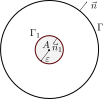
\includegraphics{figGreenMethTwoDim.pdf}
\end{figure}
\[
	\oint\limits_\Gamma \left(u \derp{v}{n}{} - v \derp{u}{n}{} \right)\, d\gamma + \oint\limits_{\Gamma_1} \left(u \derp{v}{n_1}{} - v \derp{u}{n_1}{} \right)\, d\gamma = 0
\]
\[
	v = G
\]
Нас интересует интеграл вида
\[
	\oint\limits_{\Gamma_1} \left(u \derp{G}{n_1}{} - G \derp{u}{n_1}{} \right)\, d\gamma
\]
Если интеграл берётся по окружности радиуса $\varepsilon$, то:
\[
	\derp{}{n_1}{} = - \derp{}{r}{}, \qquad dr = \varepsilon\, d\theta
\]
\[
	\iint\limits_0^{2\pi} \left( - u \derp{G}{r}{} + G \derp{u}{r}{} \right) \varepsilon d\theta = \int\limits_0^{2\pi} \left(- u \derp{w}{r}{} + w \derp{u}{r}{} + u \derp{}{r}{} \left(\ln \frac{1}{r} \right) - \ln \frac{1}{r} \derp{u}{r}{}\right) \cdot \varepsilon
\]
\[
	(- \ln r )' = - \frac{1}{r}
\]
Перейдём к пределу:
\[
	\lim\limits_{\varepsilon \to 0} \oint\limits_{\Gamma_1} \left(u \derp{G}{n_1}{} - G \derp{u}{n_1}{} \right) = \\ 
	=	\lim\limits_{\varepsilon \to 0} \int\limits_0^{2 \pi} \left(- u \derp{w}{r}{} + w \derp{u}{r}{} \right)\, d\theta - \lim\limits_{\varepsilon \to 0} \varepsilon \int\limits_0^{2 \pi} \left[u \frac{1}{\varepsilon}  + \derp{u}{r}{} \ln \varepsilon\right]\, d\theta  
\]
Так как $u, w$ --- непрерывно гладкие функции, то
\[
	\varepsilon \ln \varepsilon \underset{\varepsilon \to 0}{\to} 0
\]

В итоге получаем 
\[
	- \int\limits_0^{2 \pi} u \, d \theta
\]
Значит:
\[
	\oint\limits_\Gamma \left(u \derp{v}{n}{} - v \derp{u}{n}{} \right)\, d\gamma - \underbrace{\int\limits_0^{2 \pi} u\, d \theta}_{u(x_0, y_0) 2 \pi} = 0
\]
так как интегрируем в малой области.



